
\chapter{Results}

%First say what you are looking at. Then say what yo get from figure
%now given this what does it tell you
%for each table and figure

%{\color{red} \huge SD card not soldered \\ rest functional \\ideal implementation would be permanent\\ Will likely only encompass a days worth of data.}

\vspace{-2em}
\section{Particulate Matter}
\vspace{-2em}
\begin{figure}[!htb]
	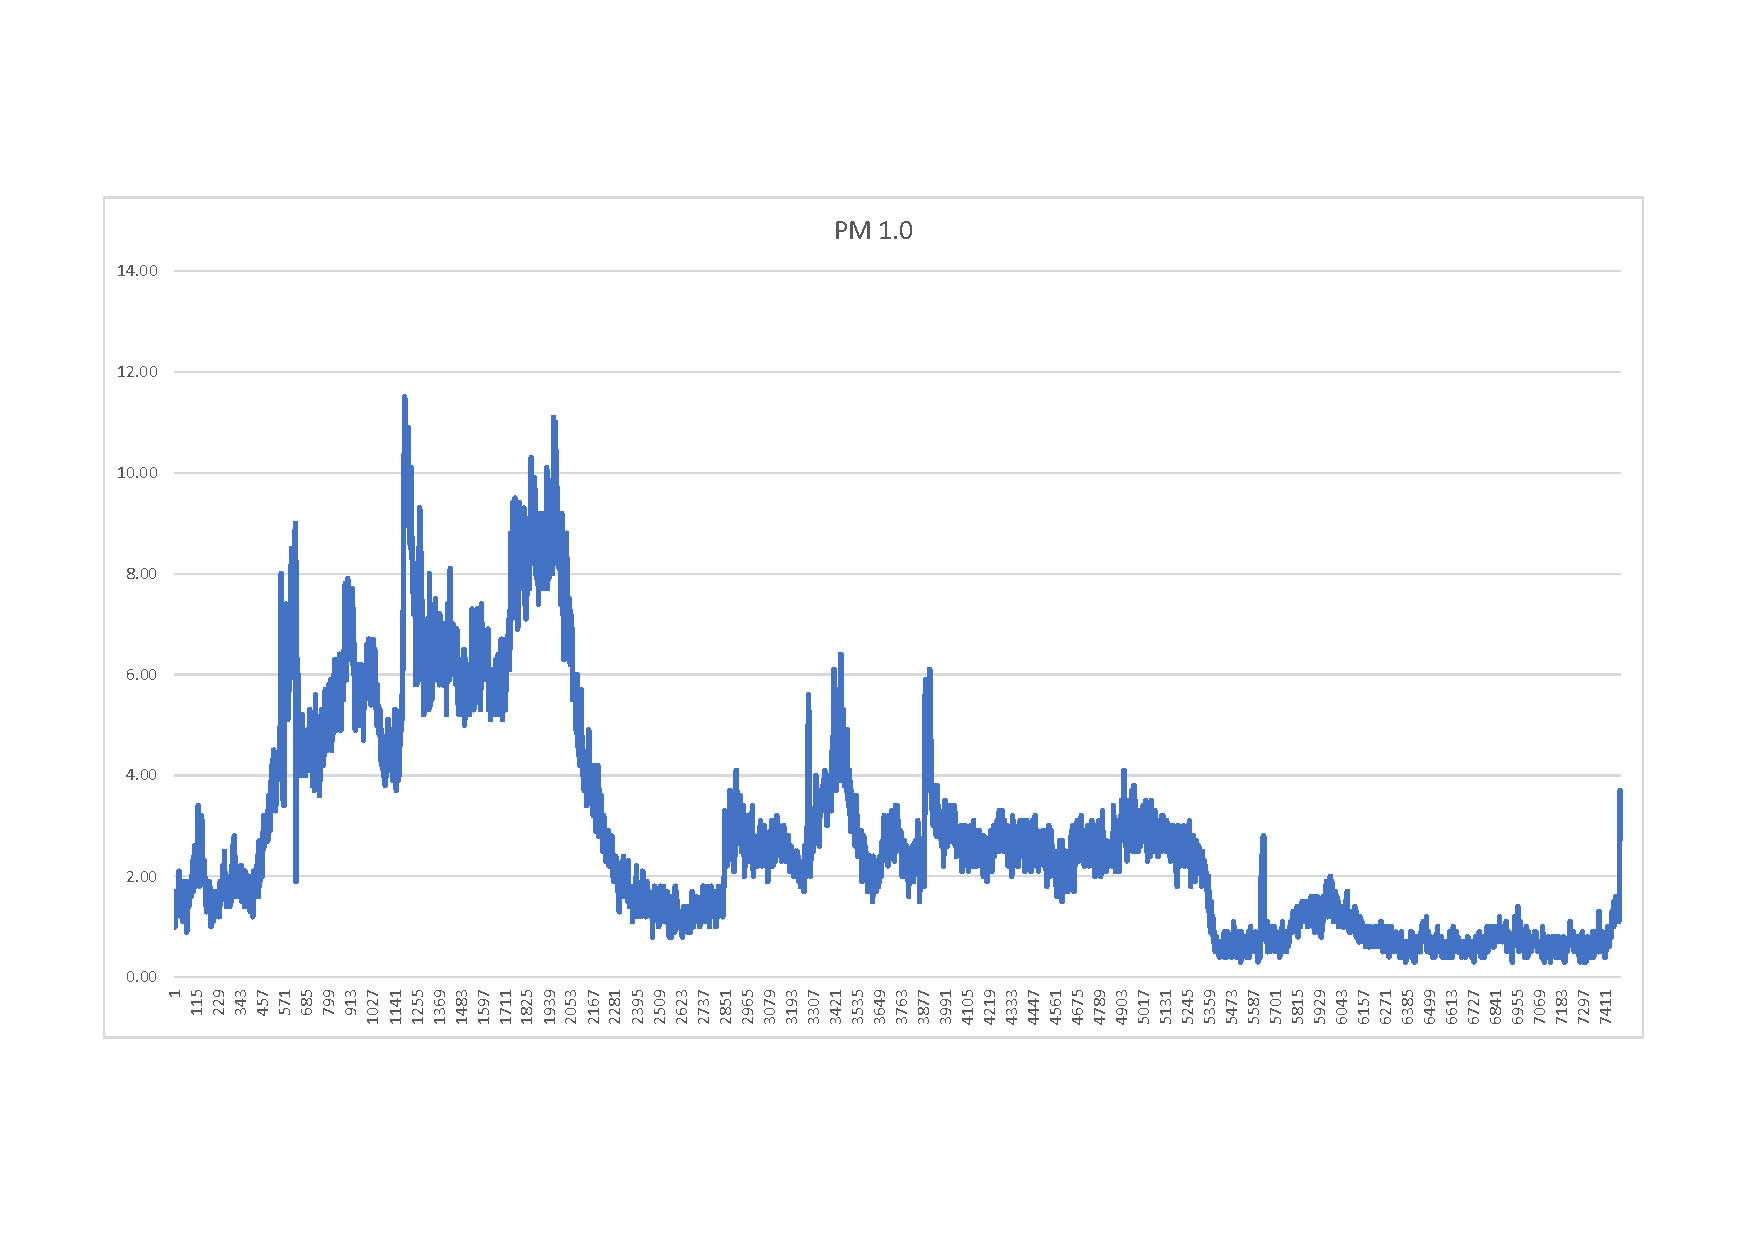
\includegraphics[width=0.45\textwidth, height = 10em]{body/fig/PM0.1.pdf}%
	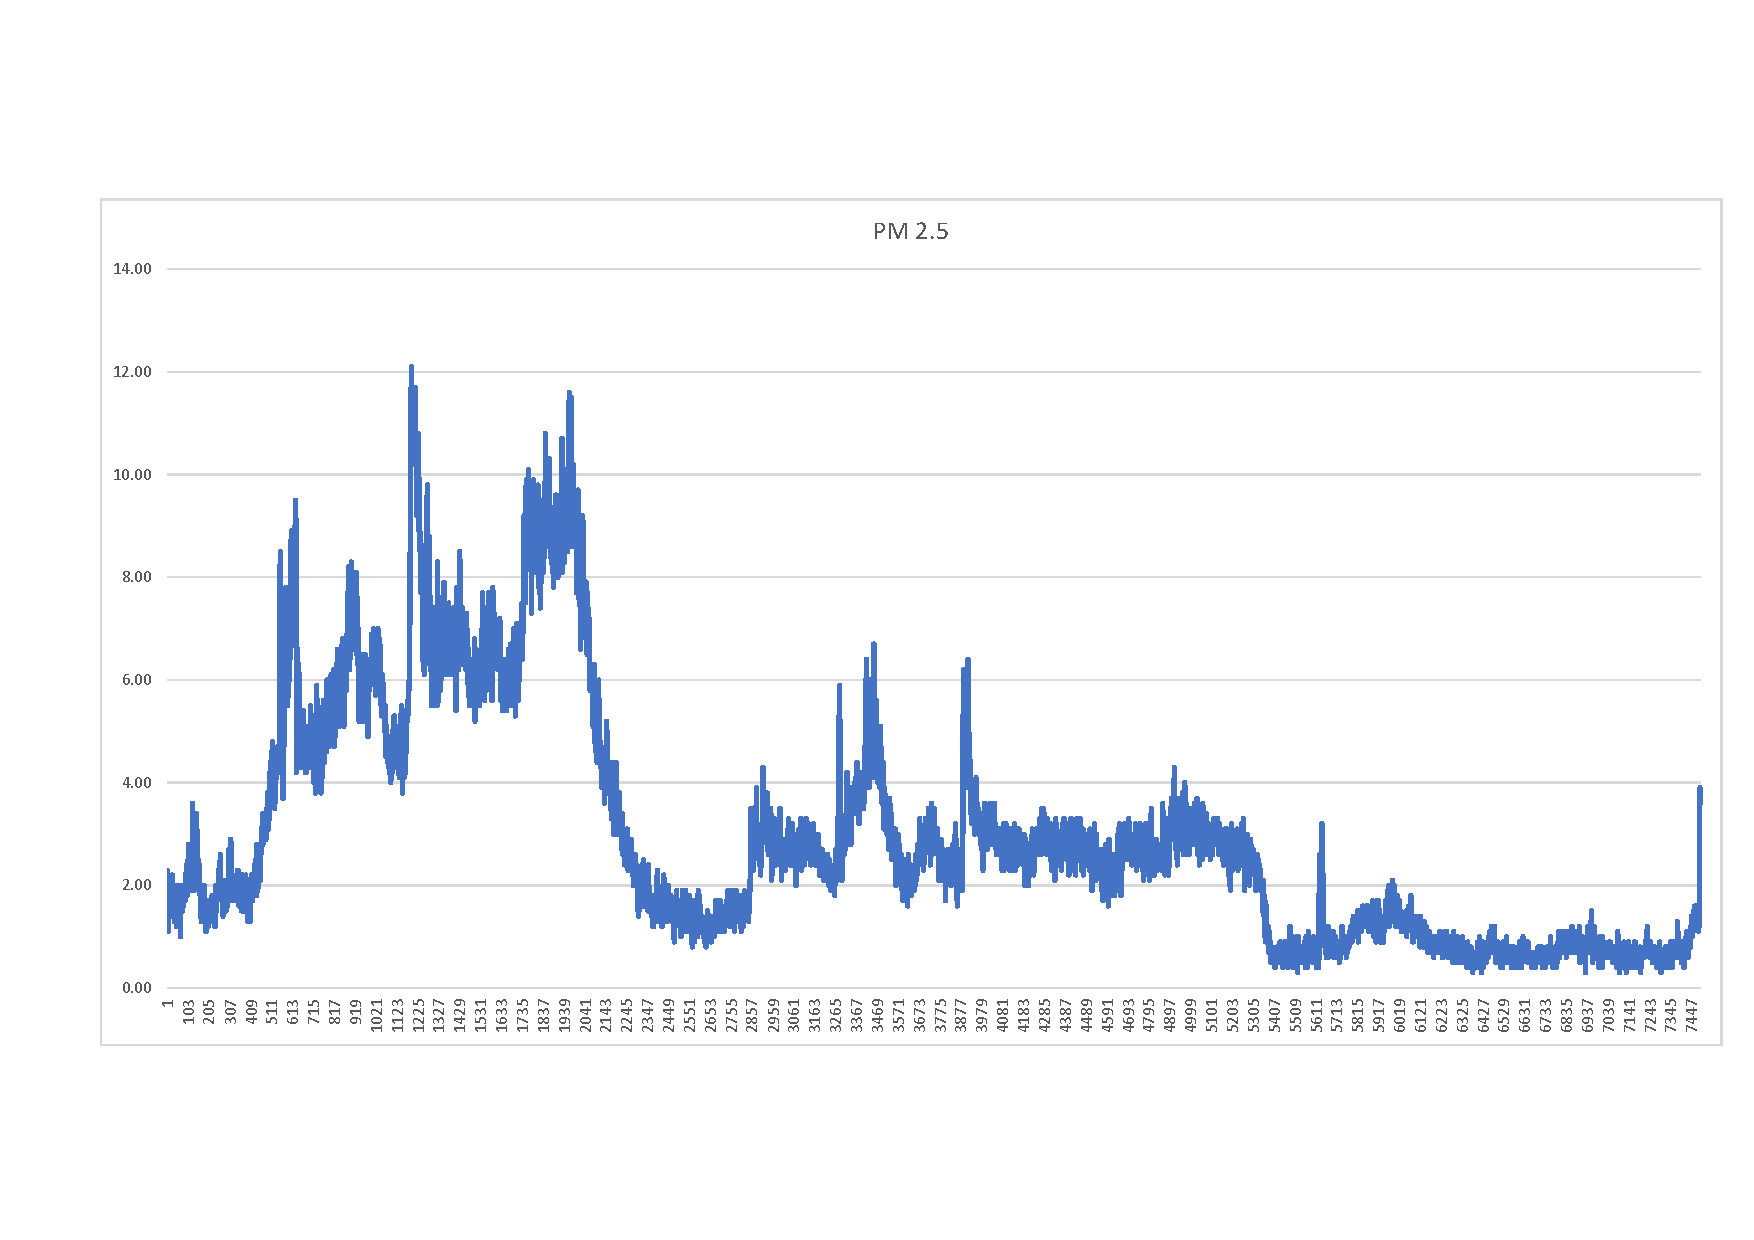
\includegraphics[width=0.45\textwidth, height = 10em]{body/fig/PM2.5.pdf}%
	\caption{PM 1.0 (left) and PM 2.5 (right)}
	\label{ACEM1}
	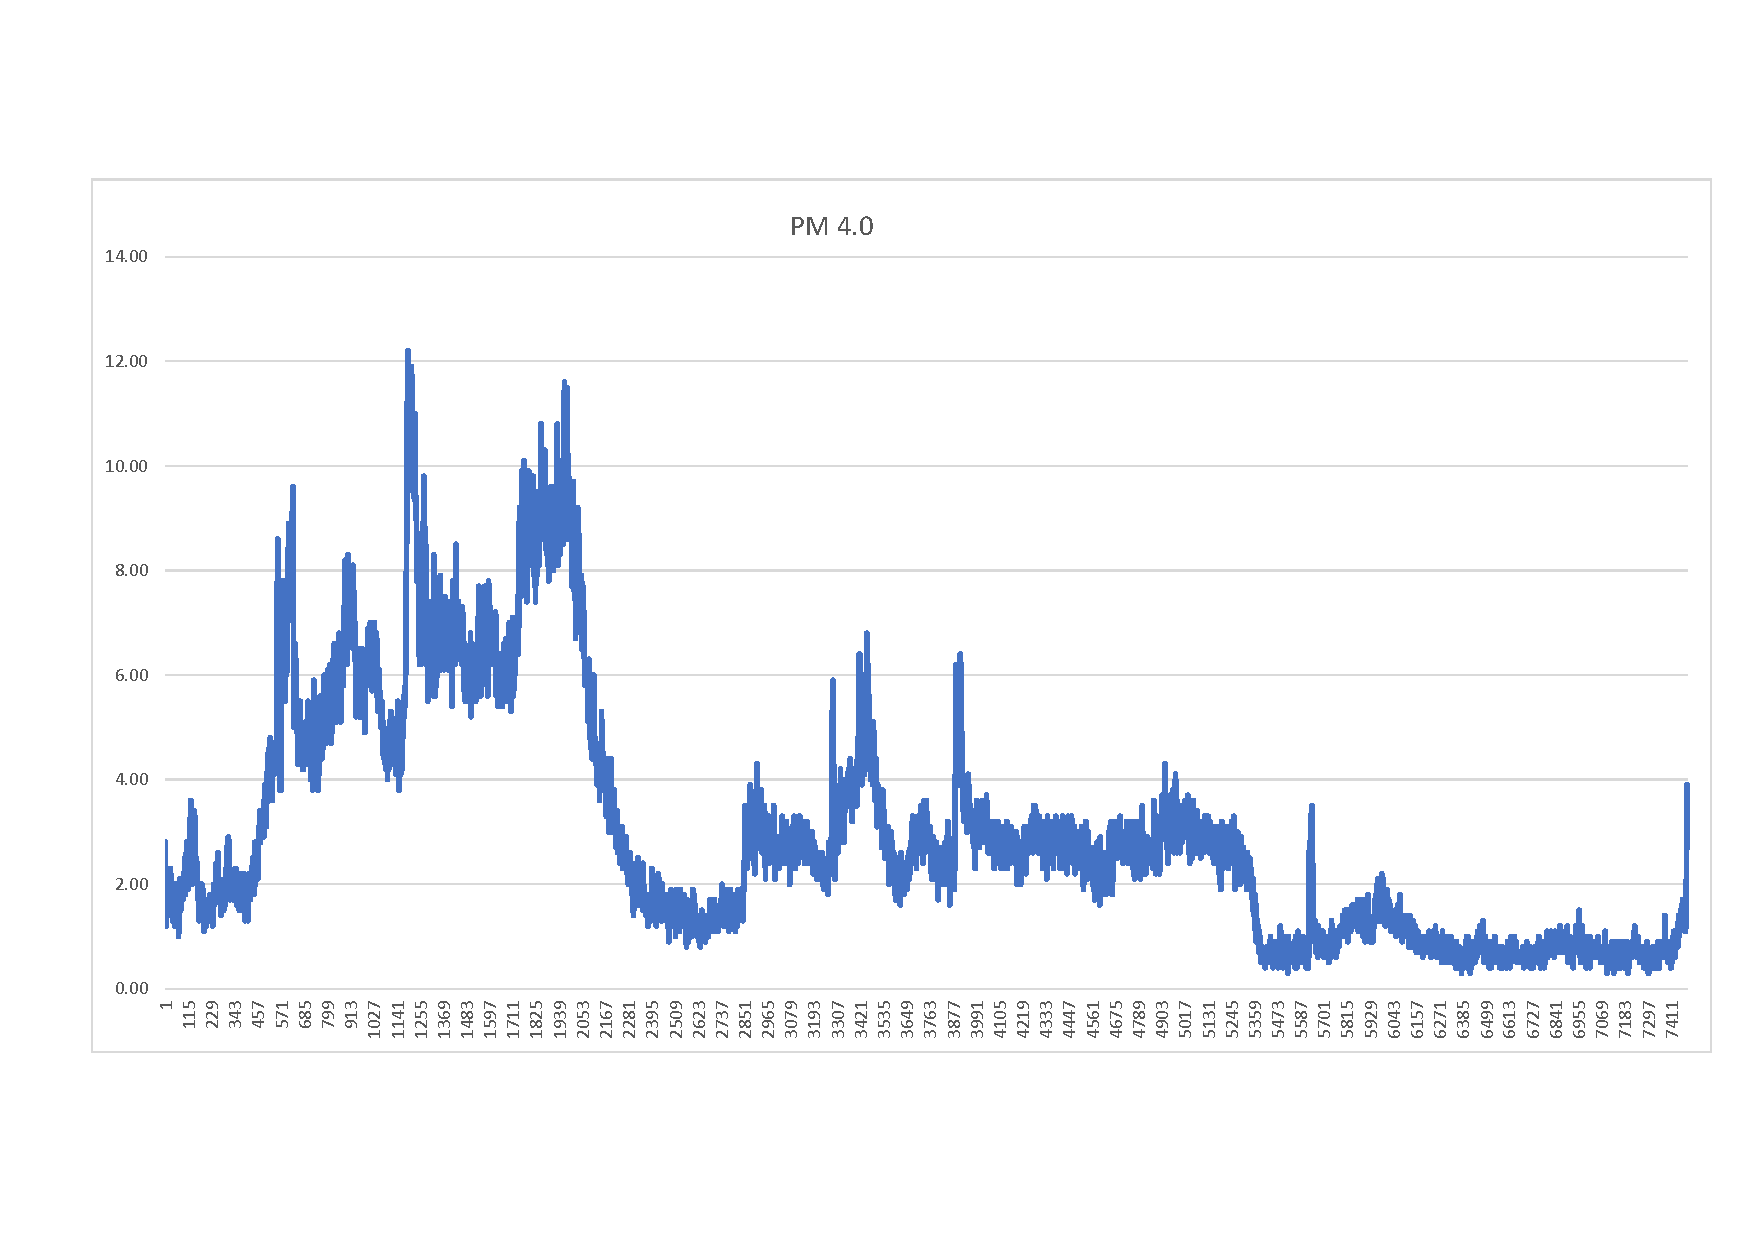
\includegraphics[width=0.45\textwidth, height = 10em]{body/fig/PM4.pdf}%
	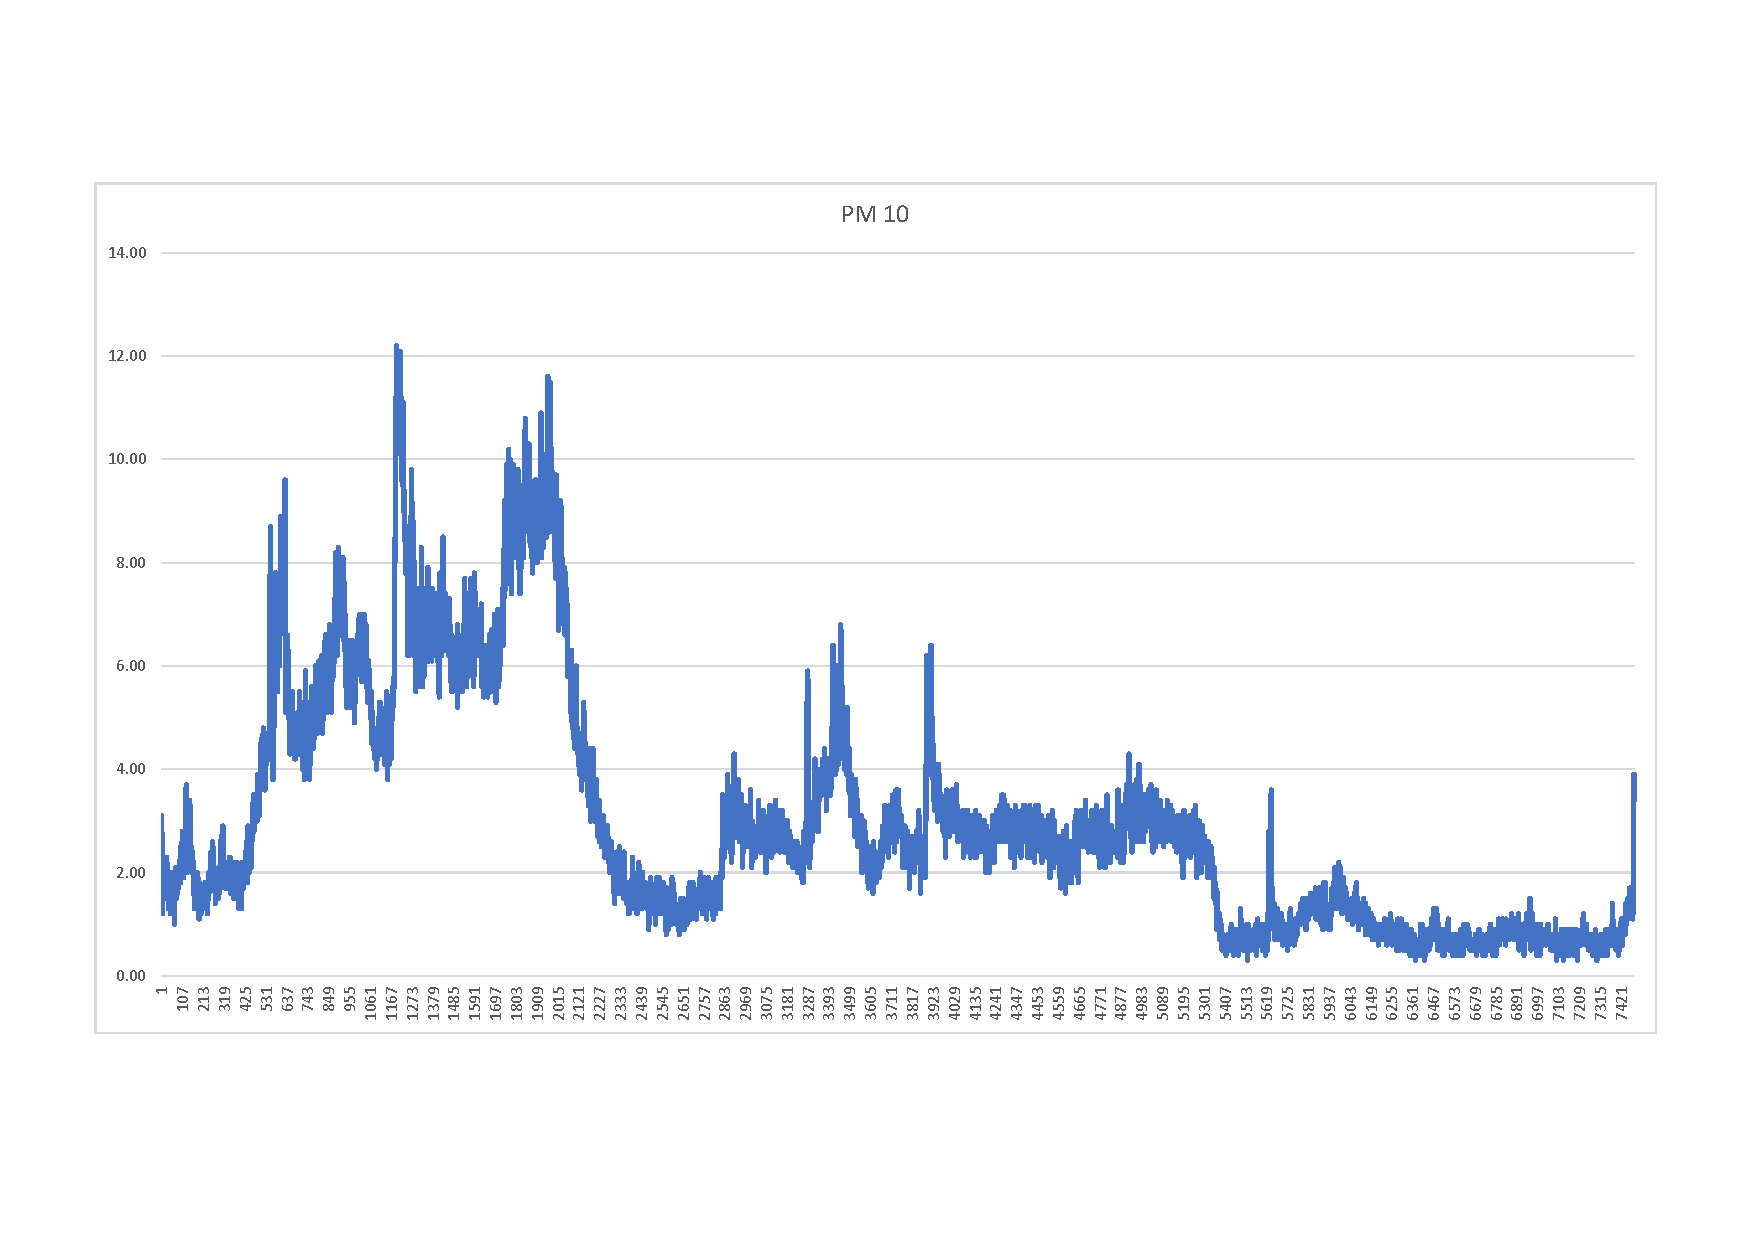
\includegraphics[width=0.45\textwidth, height = 10em]{body/fig/PM10.pdf}%
	\captionof{figure}{PM 4.0 (left) and PM 10 (right)}
	\label{ACEM2}
\end{figure}
\begin{figure}[!htb]
	\centering
	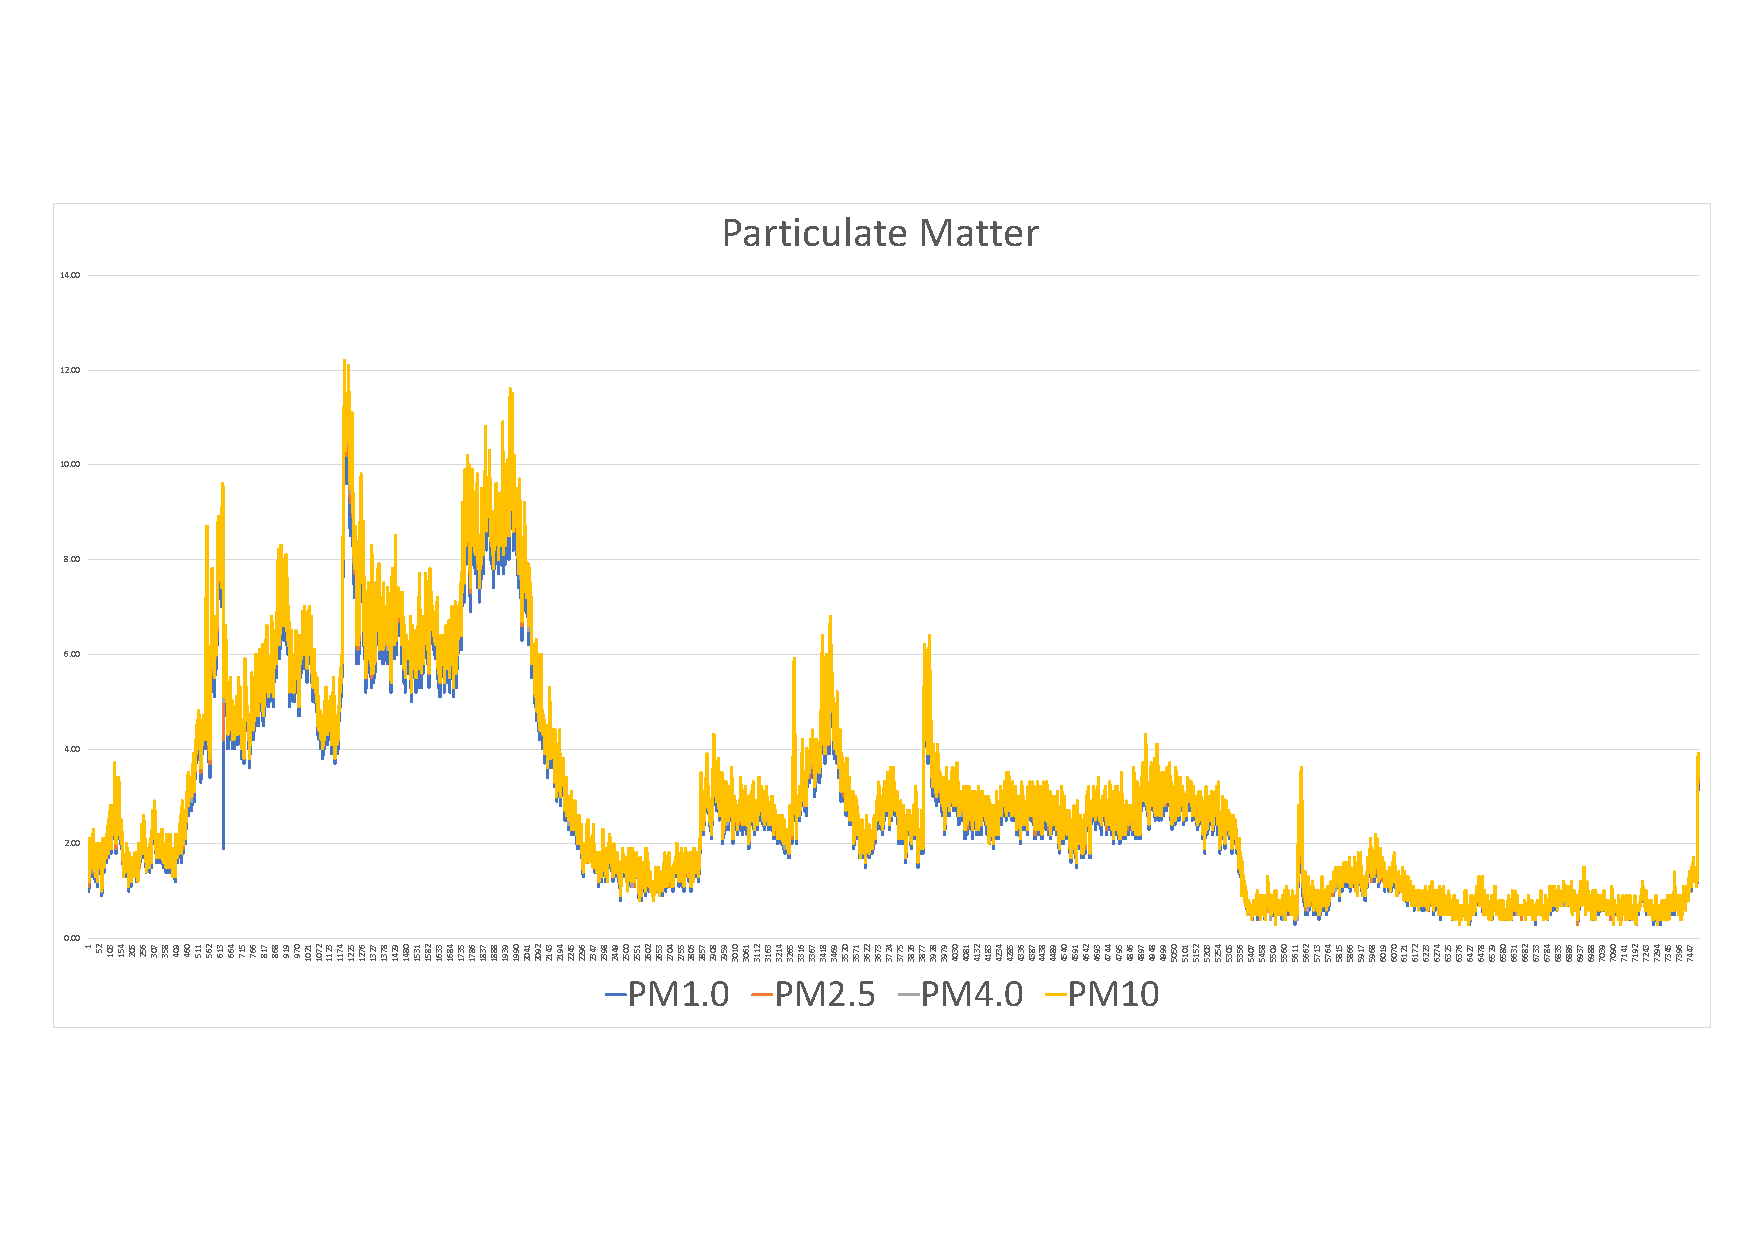
\includegraphics[width=0.7\linewidth]{body/fig/PMall.pdf}
	\caption{Part}
	\label{fig:PMall}
\end{figure}

\noindent
The correlation between all of the different types of particulate matter concentrations is rather high, as can be seen from Figure~\ref{fig:PMall}, This means we could conceivably only use the PM 2.5 reading as is the norm.




\section{CO2}
\begin{figure}[!htb]
	\centering
	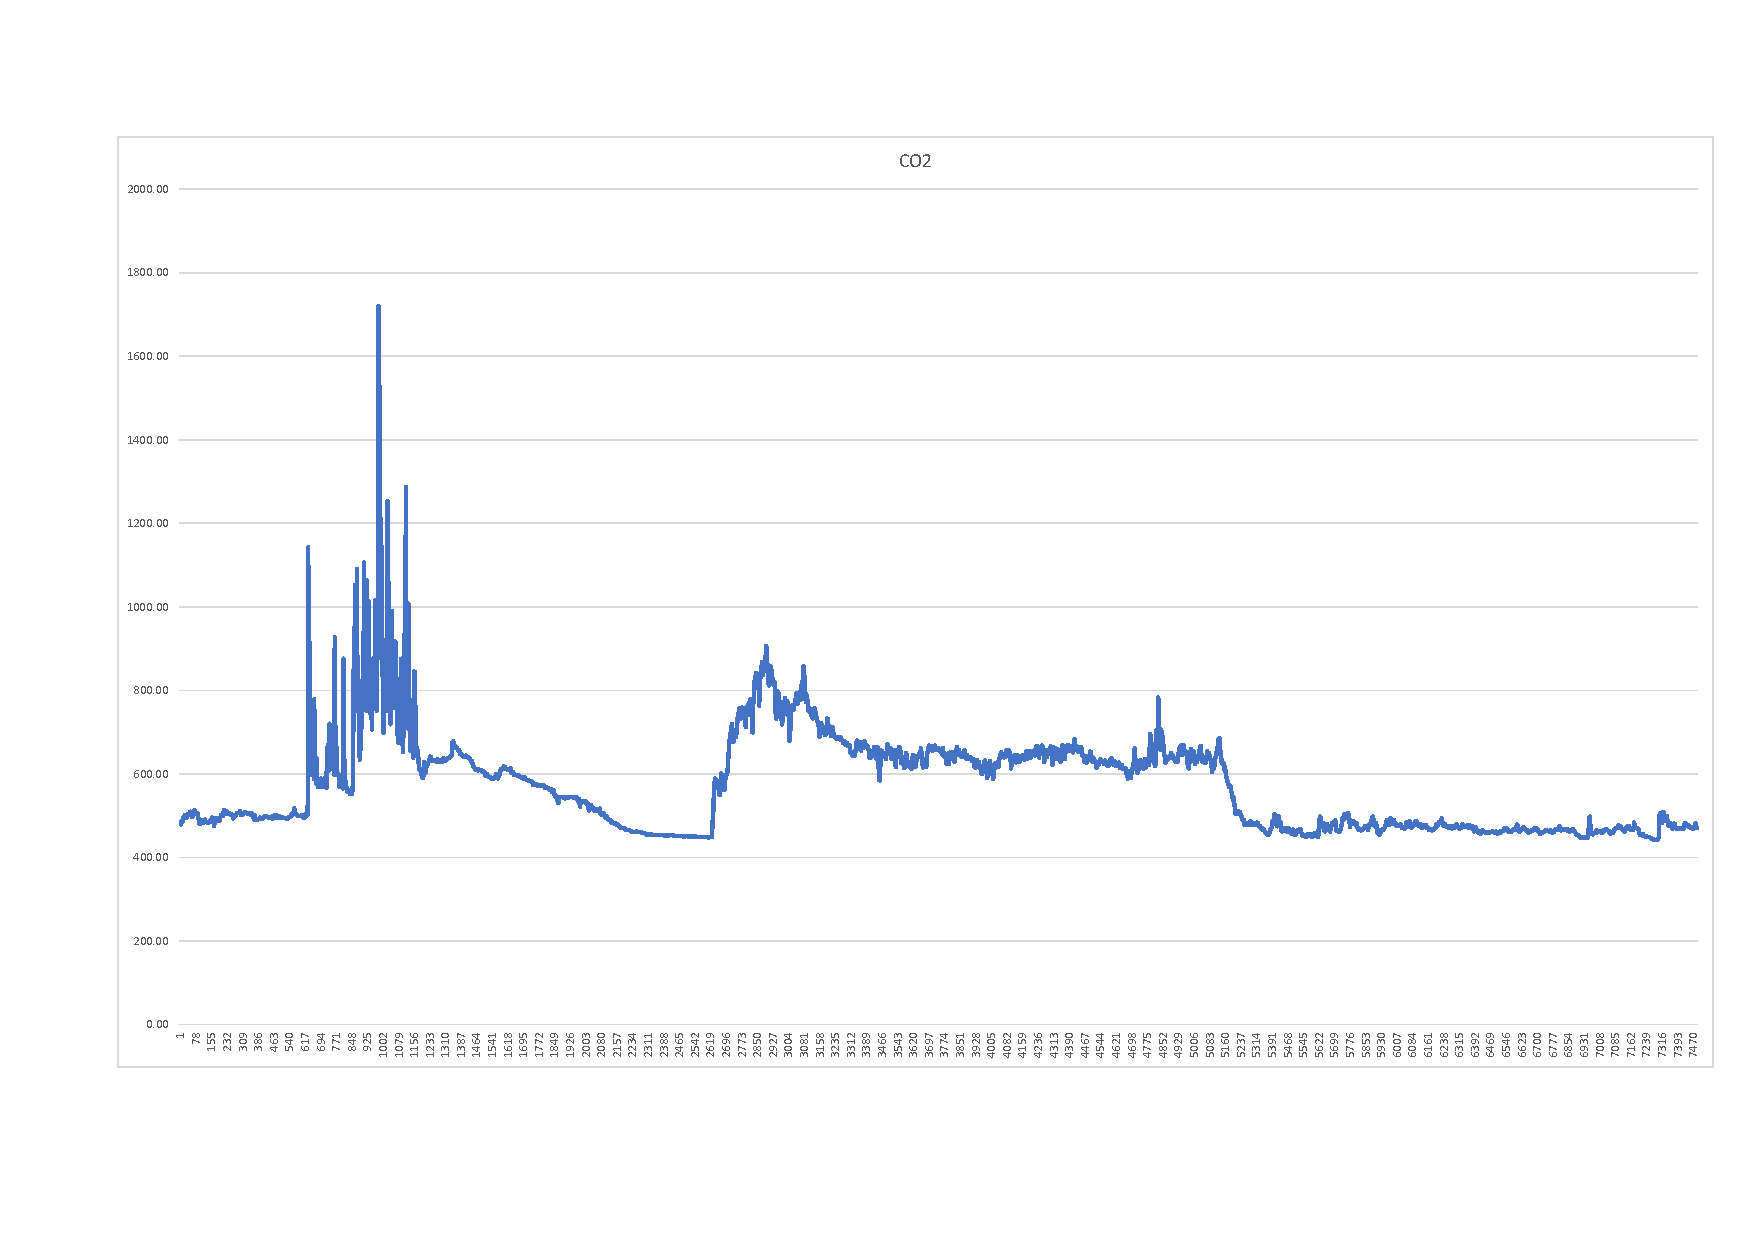
\includegraphics[width=0.7\linewidth]{body/fig/CO2}
	\caption{CO2 measurements}
	\label{fig:co2}
\end{figure}
\section{Temp and Humidity}
%\begin{figure}[!htb]
%	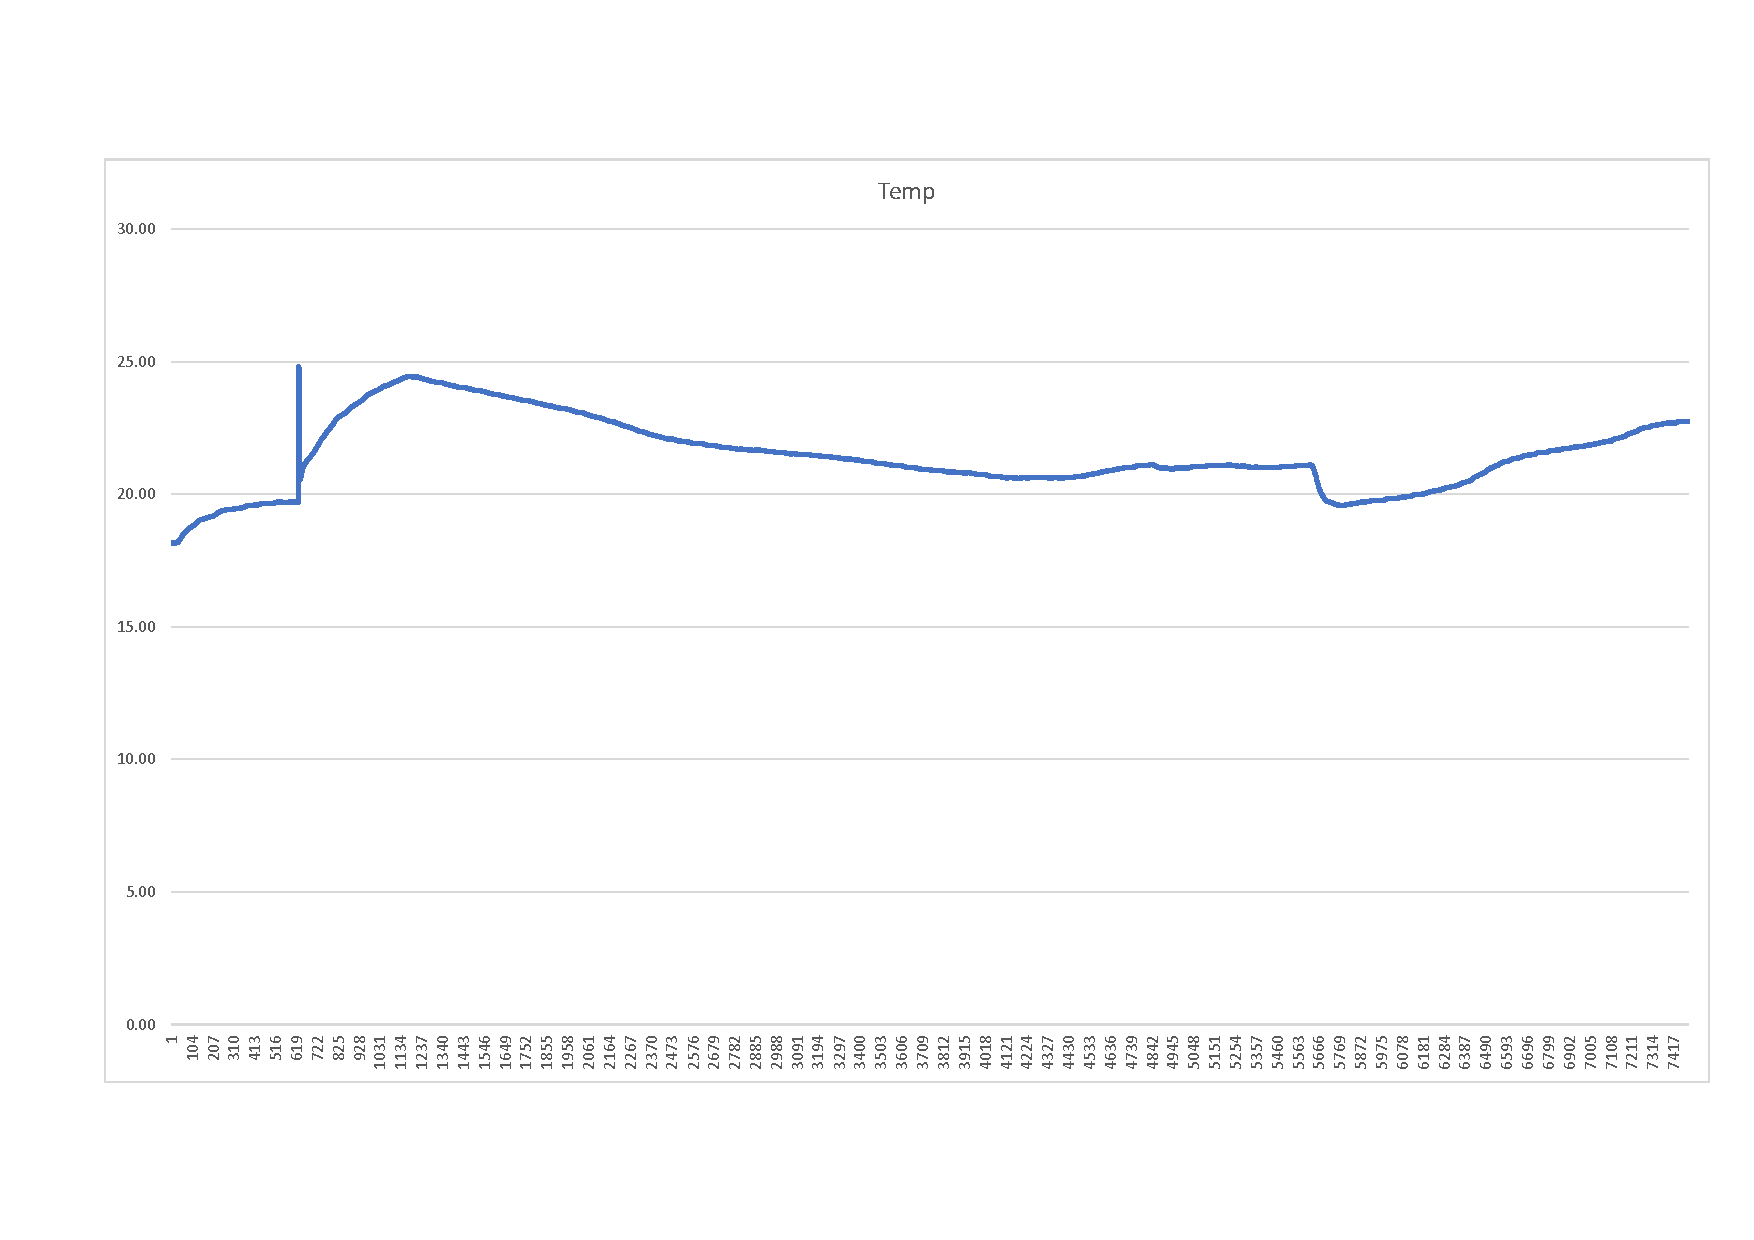
\includegraphics[width=0.5\textwidth]{body/fig/Temp.pdf}%
%	\caption{Temperature}
%	\label{fig:temp}
%	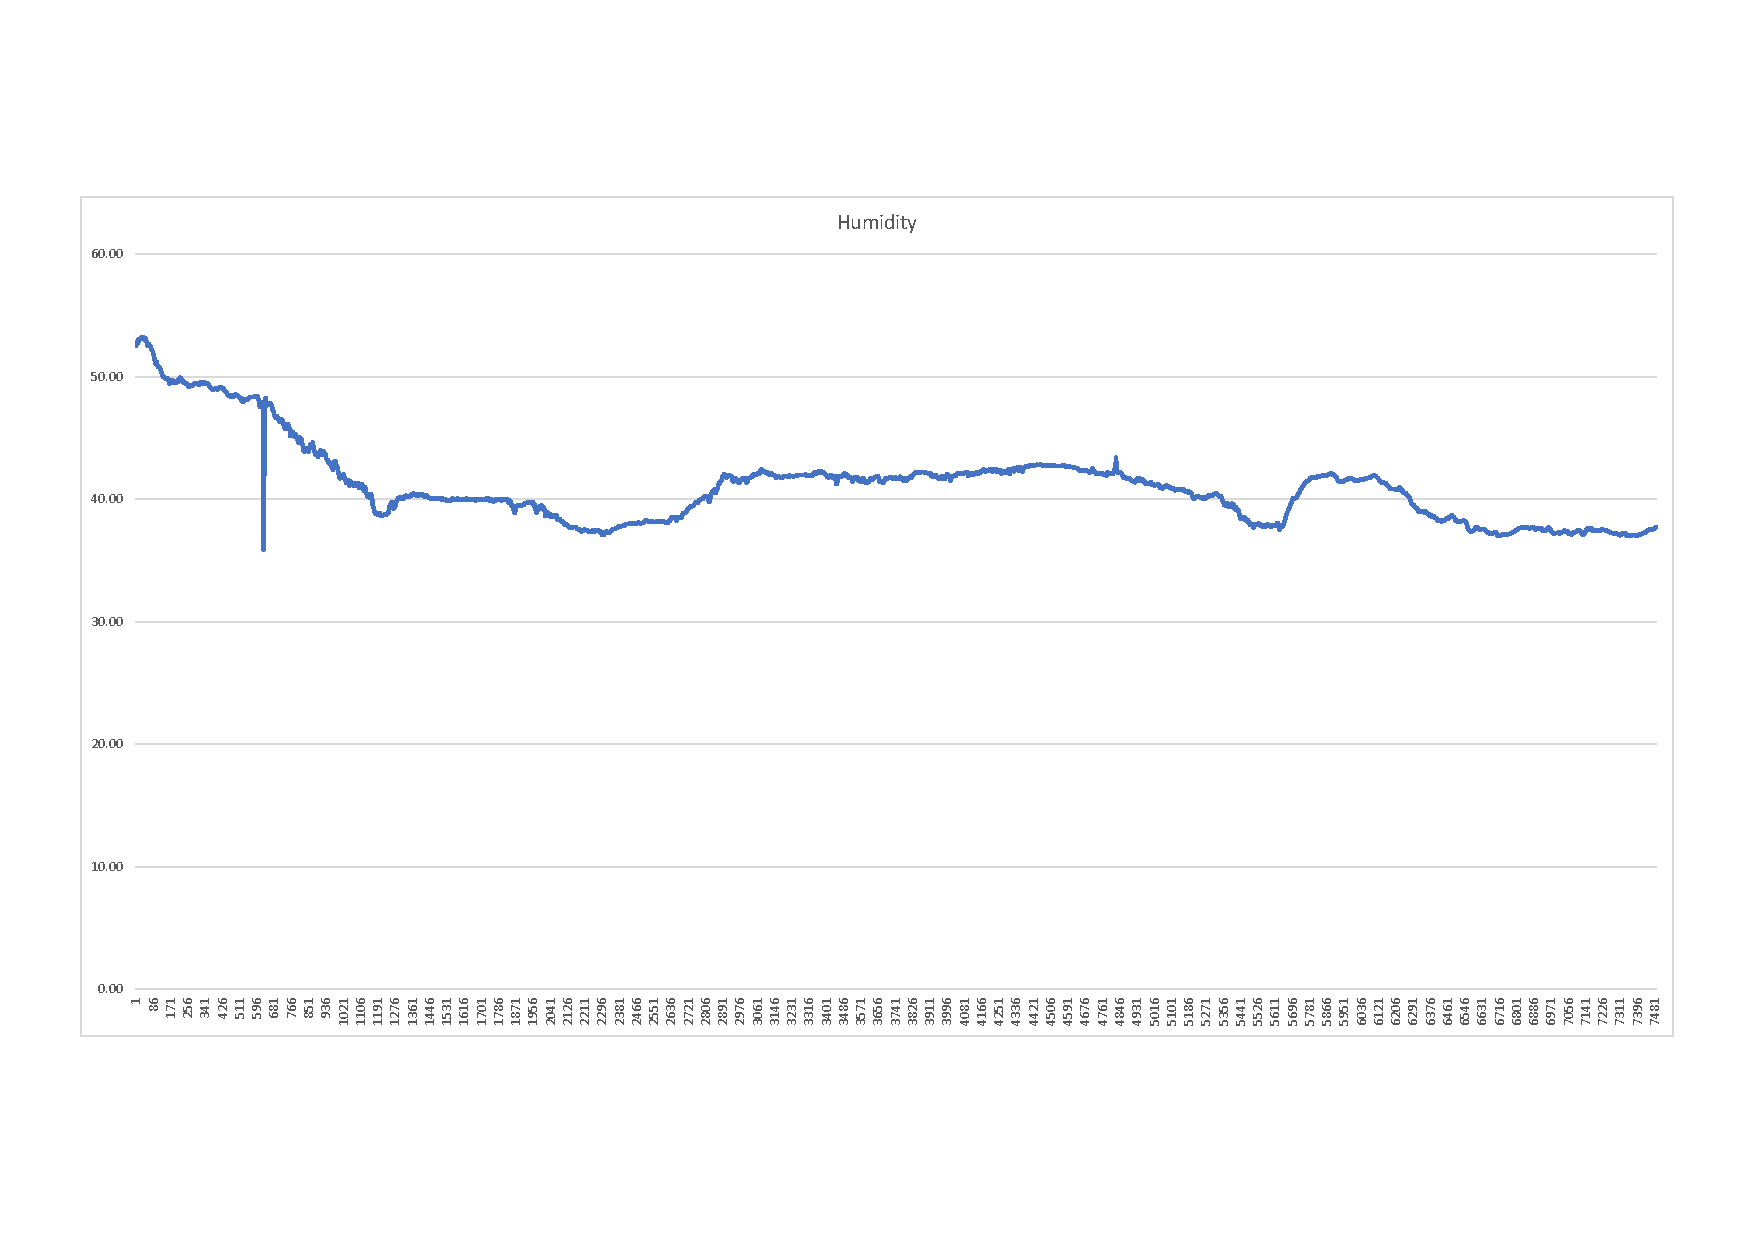
\includegraphics[width=0.5\textwidth]{body/fig/hum.pdf}%
%	\captionof{figure}{Humidity}
%	\label{fig:hum}
%\end{figure}
\begin{figure}[!htb]
	\minipage{0.45\textwidth}%
	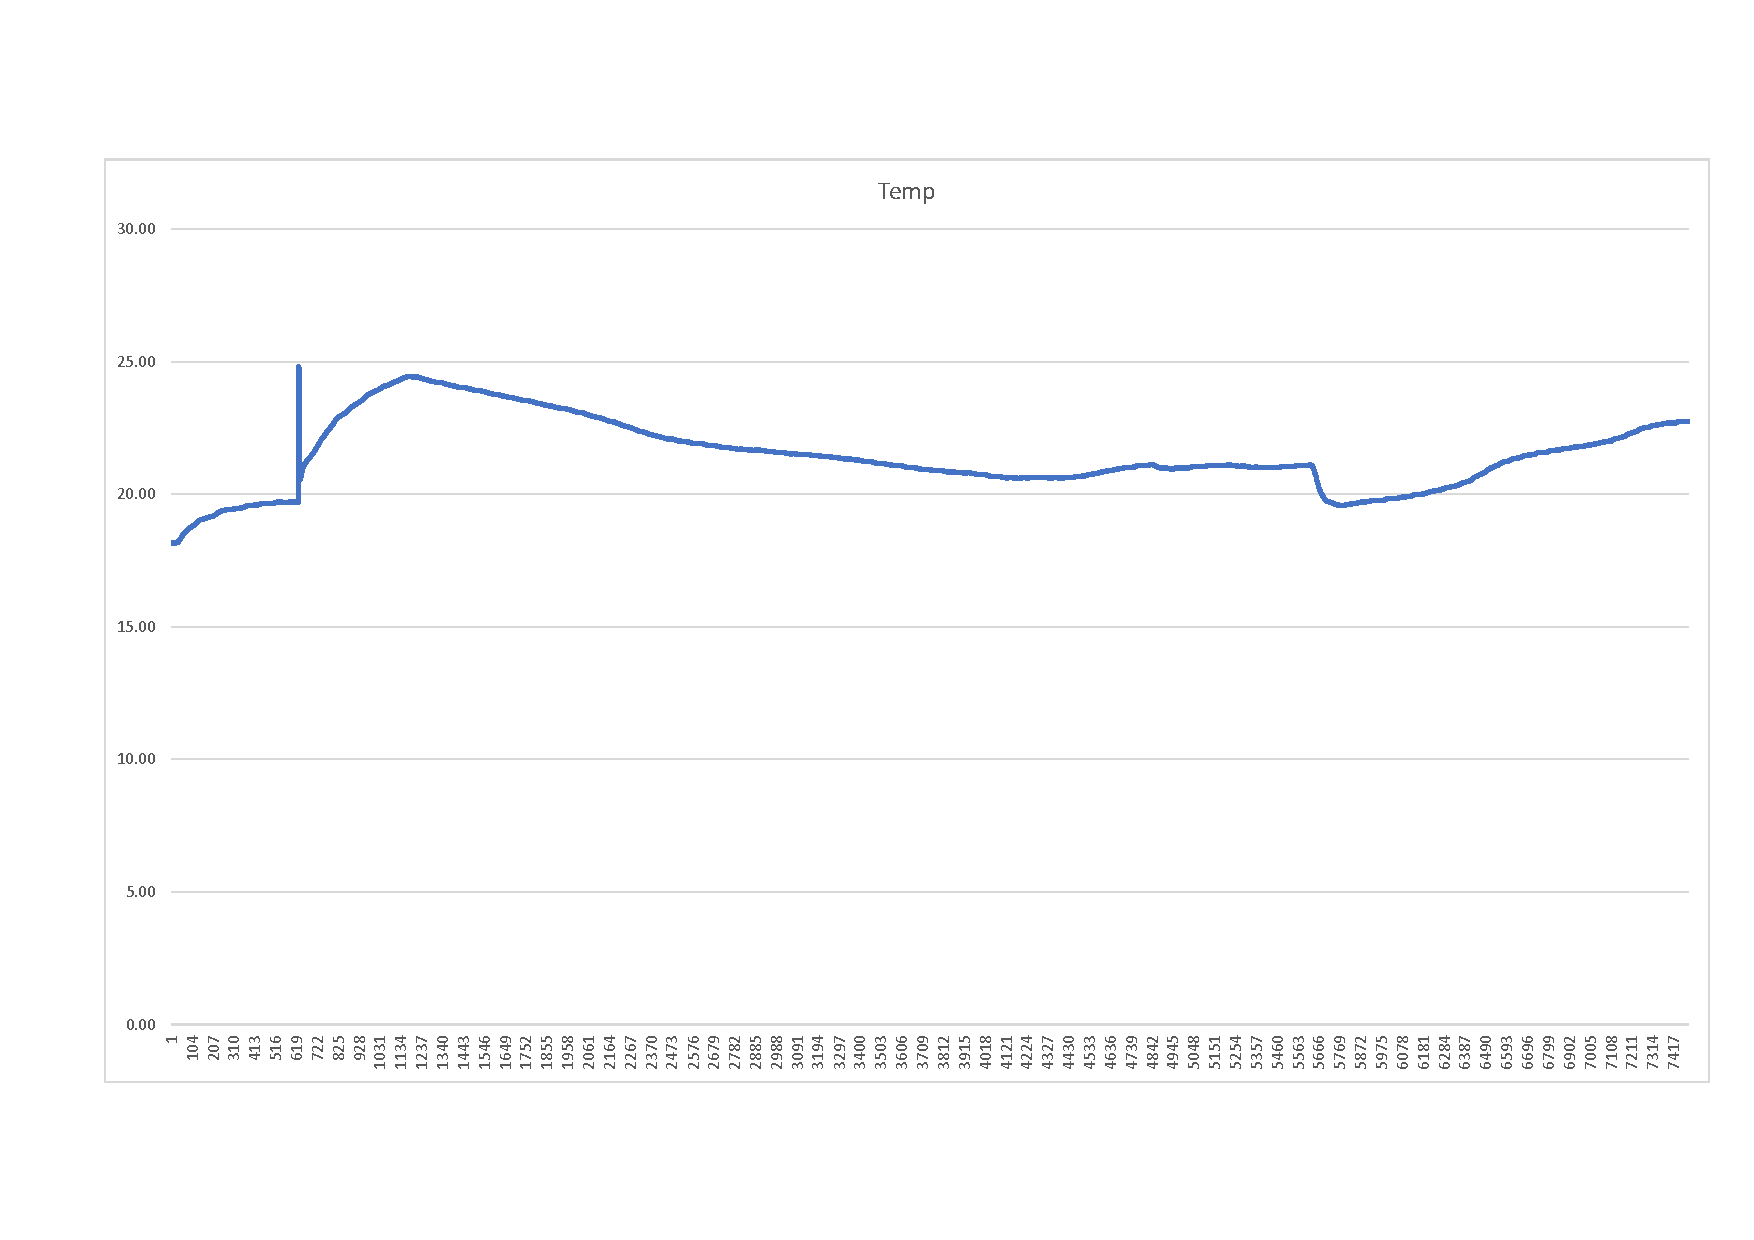
\includegraphics[width=\textwidth]{body/fig/Temp.pdf}%
\caption{Temperature}
\label{fig:temp}
	\endminipage\hfill
	\minipage{0.45\textwidth}%
	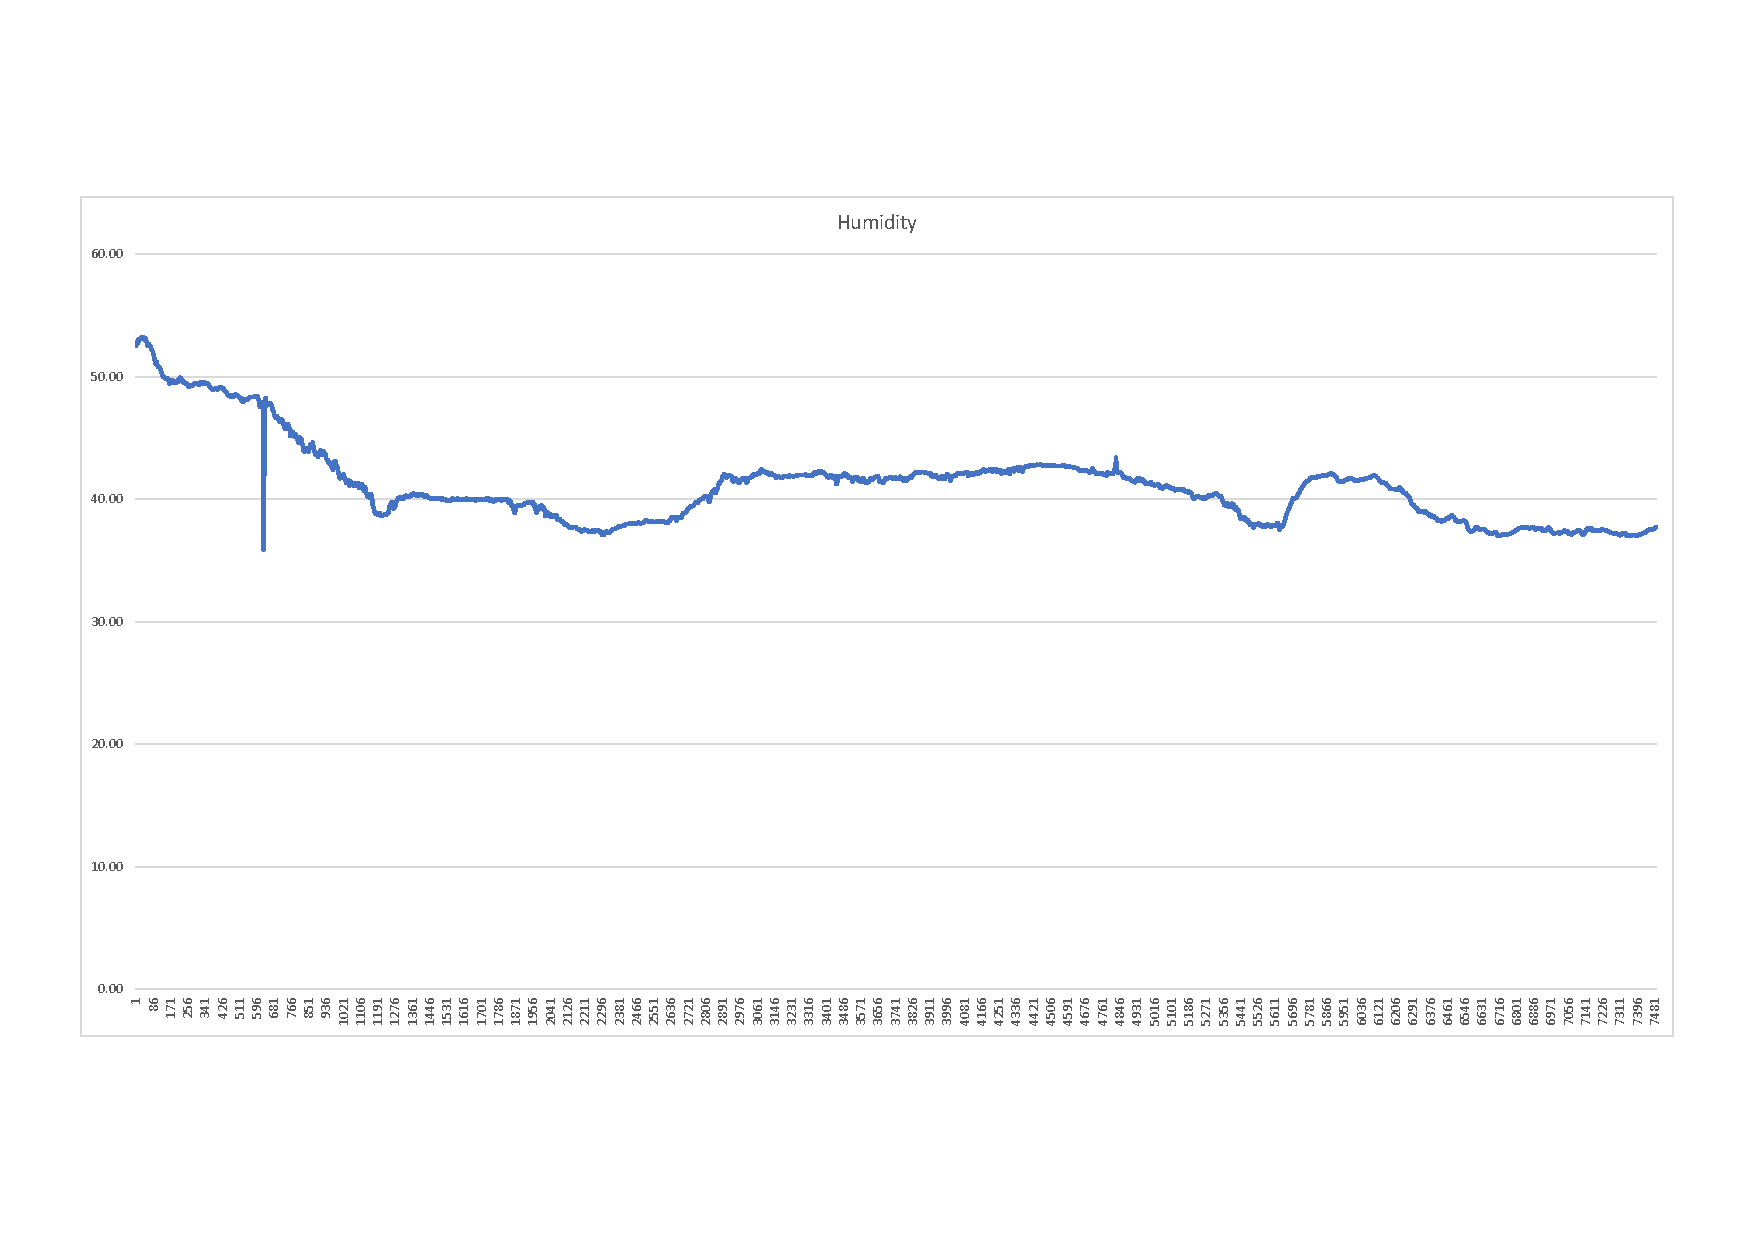
\includegraphics[width=\textwidth]{body/fig/hum.pdf}%
\captionof{figure}{Humidity}
\label{fig:hum}
	\endminipage\hfill
	
	%\text{Charts provided by \cite{2007Comparison}}
\end{figure}

\section{VOC and NOx index}
%\begin{figure}[!htb]
%	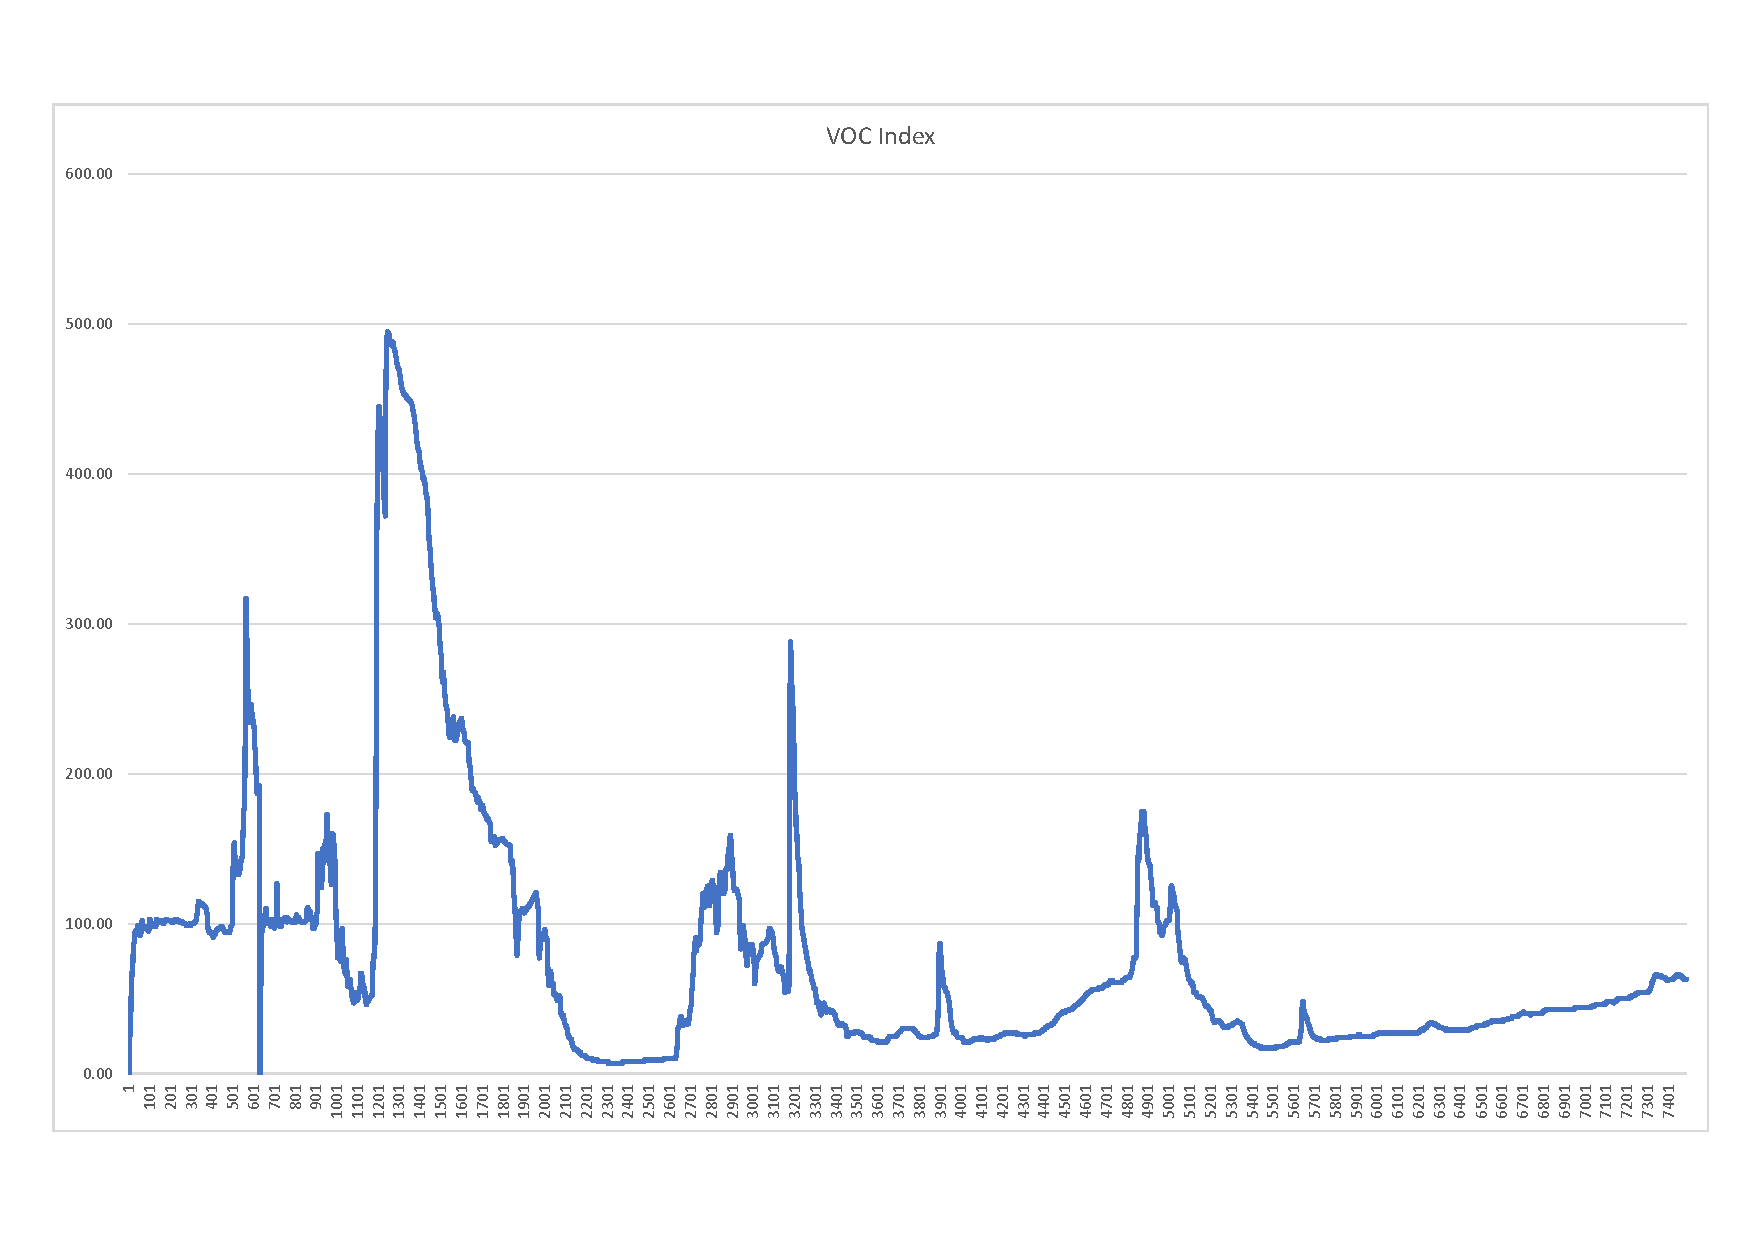
\includegraphics[width=0.5\textwidth]{body/fig/VOC.pdf}%
%	\caption{Temperature}
%	\label{fig:voc}
%	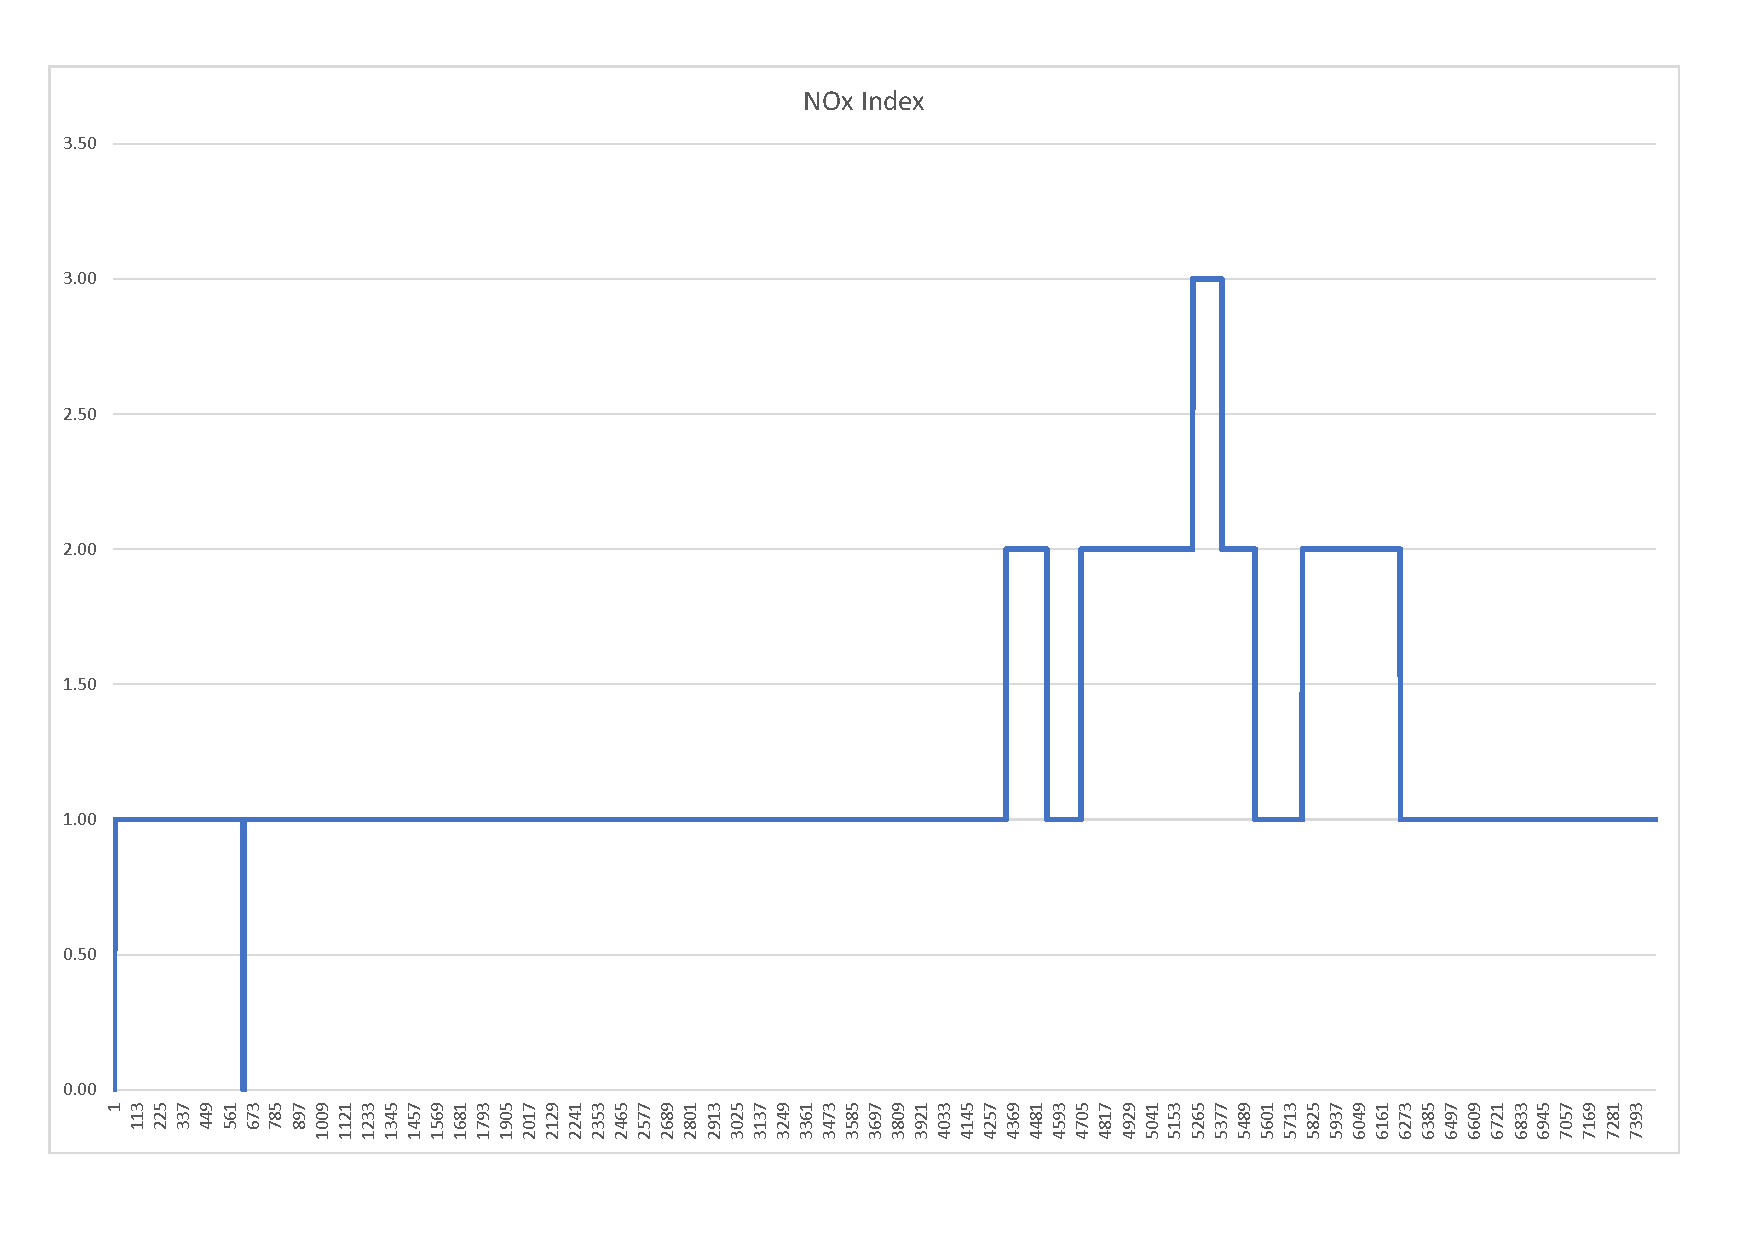
\includegraphics[width=0.5\textwidth]{body/fig/NOX.pdf}%
%	\captionof{figure}{Humidity}
%	\label{fig:nox}
%\end{figure}
\begin{figure}[!htb]
	\minipage{0.45\textwidth}%
	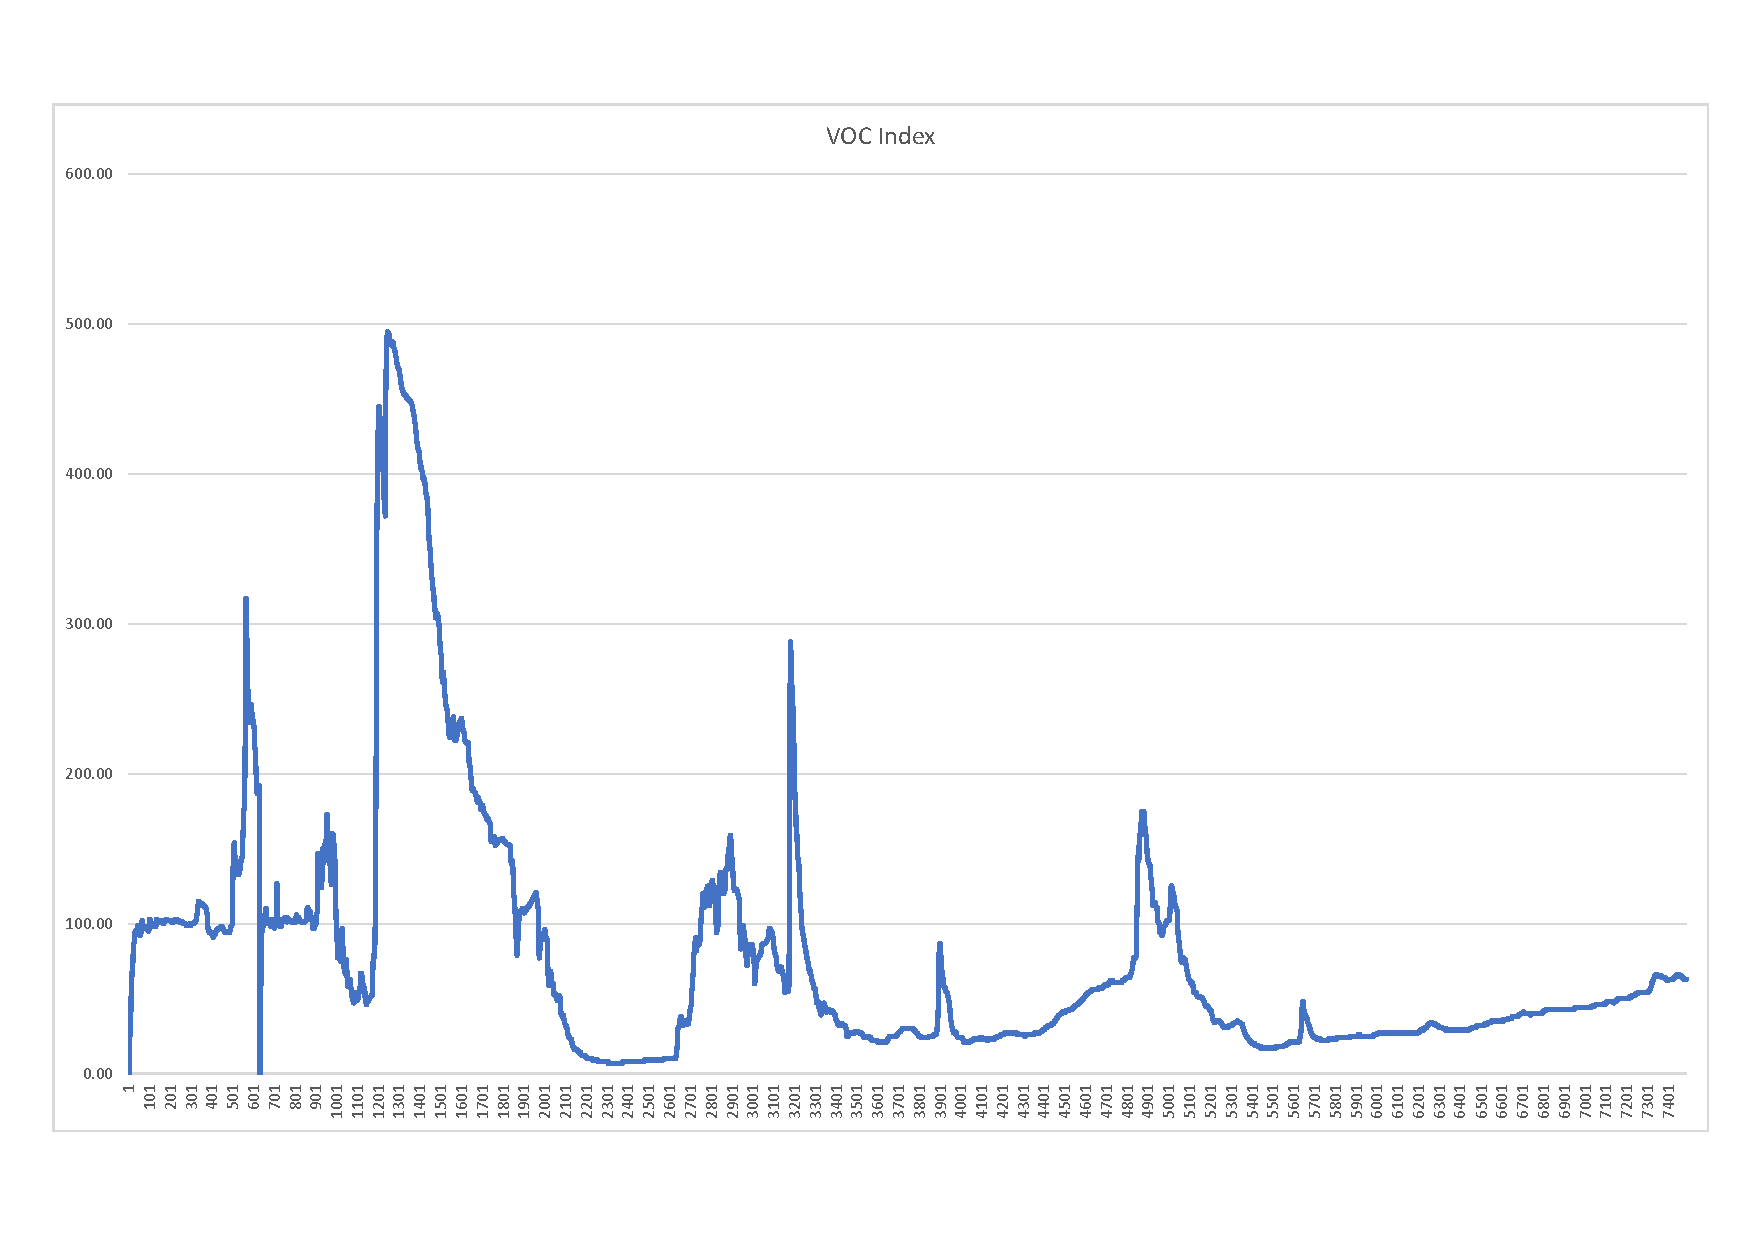
\includegraphics[width=\linewidth]{body/fig/VOC.pdf}
	\caption{VOC}\label{fig:voc}
	\endminipage\hfill
	\minipage{0.45\textwidth}%
	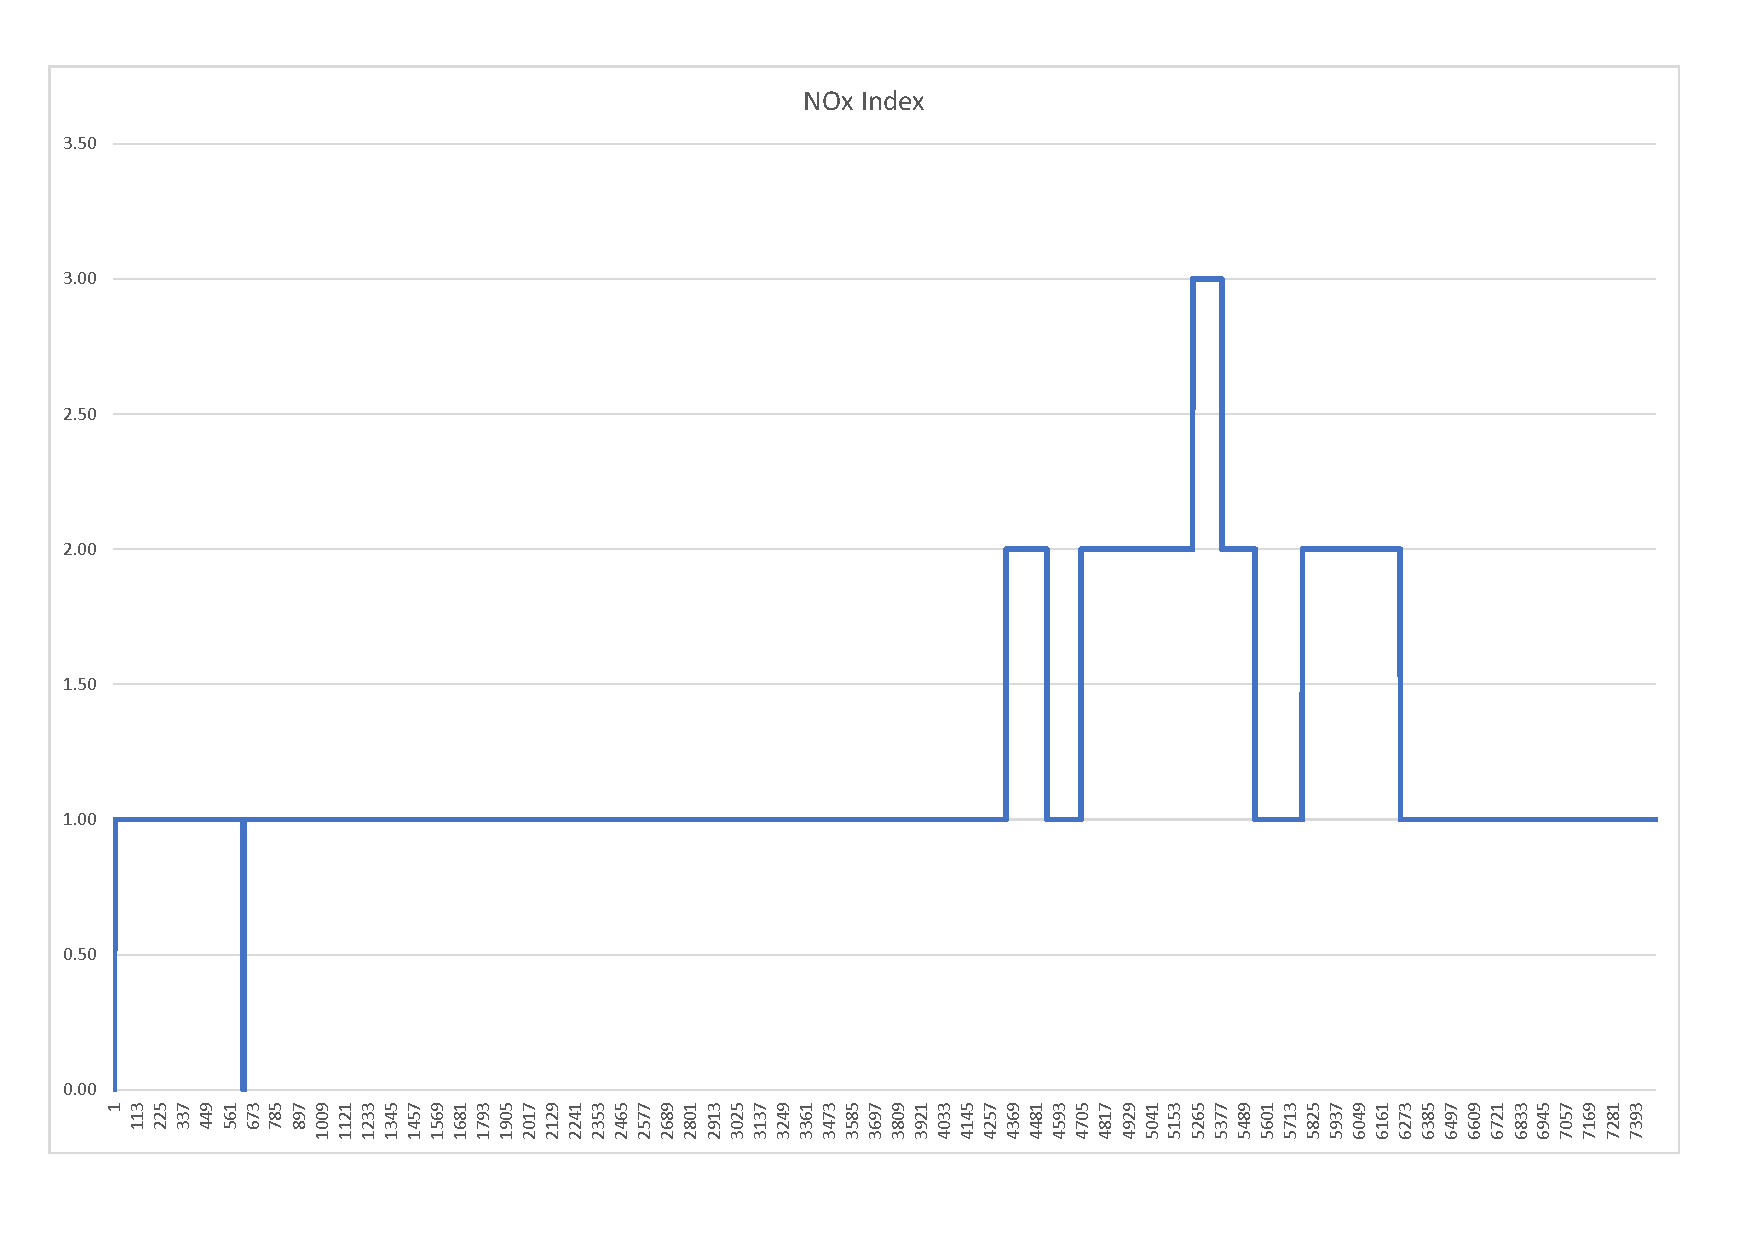
\includegraphics[width=\linewidth]{body/fig/NOX.pdf}
	\caption{NOx}\label{fig:nox}
	\endminipage\hfill

	%\text{Charts provided by \cite{2007Comparison}}
\end{figure}

